\section{Statistical analysis}
\label{sec:approach}

\subsection{Data selection}
\label{sec:halos:data}


In this work we use the 4FGL-DR4 catalog~\cite{2022ApJS..260...53A, 2023arXiv230712546B}. We group the known types of associated sources into two classes:%
\footnote{Cf. table 5 in ref.~\cite{2022ApJS..260...53A} for details about the types of sources. Galactic sources: psr, hmb, sfr, snr, pwn, gc, gal, bin, msp, lmb, spp, glc, nov. Extragalactic sources: bll, sbg, rdg, css, bcu, ssrq, fsrq, sey, nlsy1, agn.}
\begin{itemize}
    \item Galactic \new{(dominated by millisecond pulsars at high latitudes~\cite{smith2023third, 2020ApJS..247...33A, Fornasa:2015qua, Hooper:2024avz, Cholis:2014noa, Caraveo:2013lra})}: pulsars, binaries, star-forming regions, supernova remnants, pulsar wind nebulae, globular clusters, and novae;
    \item Extragalactic (\new{mostly AGNs~\cite{fossati1998unifying, 2020ApJS..247...33A, Fornasa:2015qua, Dermer:2009zz, Ackermann_2015, Ajello:2015mfa, Lisanti:2016jub}}): blazars, quasars, starburst galaxies, normal galaxies, radio galaxies and radio sources, Seyfert galaxies, and non-blazar active galaxies.
\end{itemize}
%
%% aure: working here
%
\new{This choice is made to group sources based on their fundamentally different physical origins and radiation environments. By separating the magnetospheric emission characteristic of Galactic pulsars from the jet-driven processes of extragalactic AGNs, we ensure that the classification reflects the intrinsic physical diversity of the $\gamma$-ray sky, which manifests in distinct spectral signatures.}

In order to characterise the sources, we focus on their energy spectra modeled with the log-parabola (LP) function
\be
\label{eq:log_par}
\ln \frac{F(E)}{K} = - \alpha \ln \frac{E}{E_0} - \beta \left(\ln \frac{E}{E_0} \right)^2,
\ee
where the parameters correspond to the following columns in the 4FGL-DR4 catalog:
$K$ -- \texttt{LP\_ Flux\_Density},
$\alpha$ -- \texttt{LP\_Index},
$\beta$ -- \texttt{LP\_beta},
and $E_0$ -- \texttt{Pivot\_Energy}.
%
\\
\new{The LP model provides a well-motivated spectral choice; it offers a significant improvement over a simple power law, as evidenced in the \texttt{LP\_SigCurv} column in the 4FGL-DR4 catalog, and performs at least as well as a power law with exponential cut off both for the unassociated and for the associated Galactic and extragalactic sources (figure~\ref{fig:LP_vs_PLEC}).} \old{At the same time, it avoids the complexity and statistical weaknesses of using high-dimensional binned fluxes.} 


\begin{figure}
    \centering
    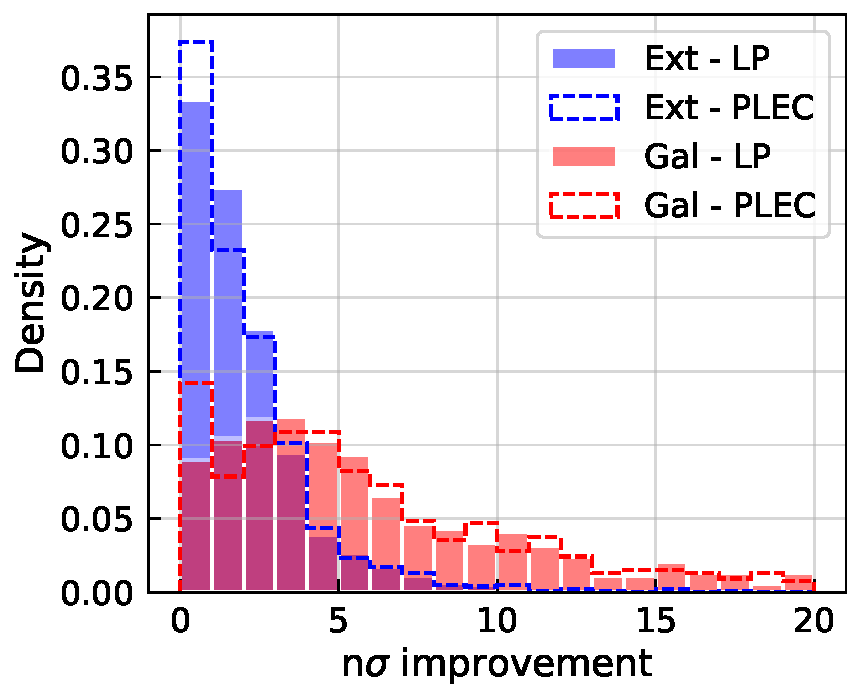
\includegraphics[width=0.45\linewidth]{sections/paper_dm_halos/img/LP_vs_PLEC/nsigma_LP_PLEC.pdf}
    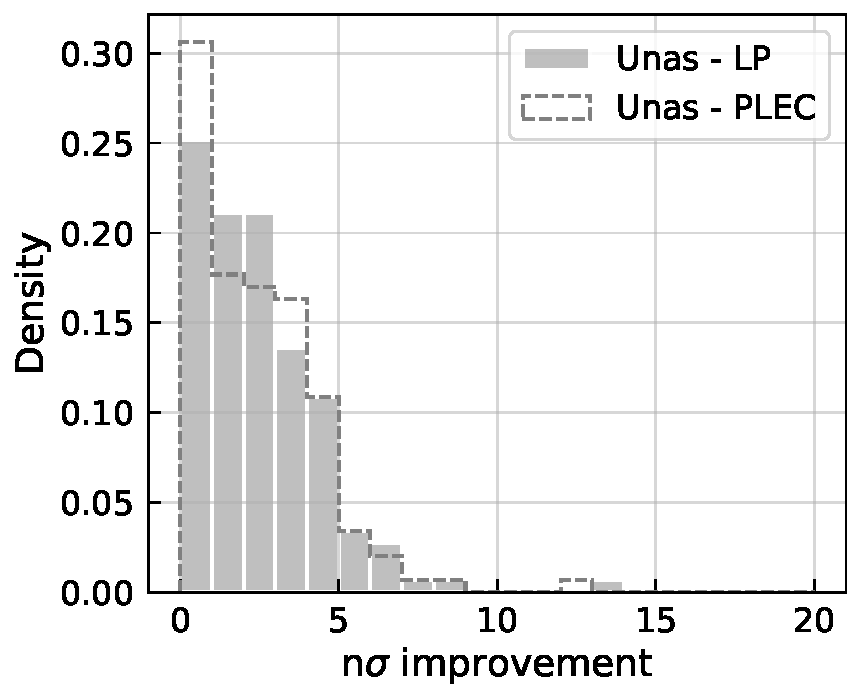
\includegraphics[width=0.45\linewidth]{sections/paper_dm_halos/img/LP_vs_PLEC/nsigma_LP_PLEC_unas.pdf}
    \caption{\new{Distribution of the significance of fit improvement, as reported in the 4FGL-DR4 catalog, when replacing a power-law energy spectrum with either a log parabola (LP) or a power law with an exponential cutoff (PLEC). We display the histograms for associated sources ({left} panel) and unassociated sources ({right} panel).}}
    \label{fig:LP_vs_PLEC}
\end{figure}
%
Provided that only three parameters are independent and that $E_0$ in the catalog is different for different sources, we rescale $E_0$ to a fixed value of 1 GeV (for analysis of $\mdm> 20$ GeV) or 100 MeV (for $\mdm < 20$ GeV). 
We use the following three parameters as input features:

\ben
\item 
$\log_{10}\phi$ -- the logarithm of the
 flux integrated between 100 MeV and 1 TeV (obtained by summing fluxes in energy bins provided in the catalog);
\item 
$\alpha$ -- \texttt{LP\_Index} rescaled to $E_0 = 1$ GeV or $E_0 = 100$ MeV depending on the choice of DM mass, i.e., above or below 20 GeV respectively;
\item
$\beta$ -- \texttt{LP\_beta}.
\een
We collect these variables for each source $i$ inside a vector ${\bx}_i\equiv \{\log_{10}(\phi_i), \alpha_i, \beta_i\}$.
%
In our analysis, we consider only sources with Galactic latitudes $|b| > 10^\circ$.


\subsection{Covariate and prior shifts}
\label{sec:cov_prior}


\begin{figure}
    \centering
    
\includegraphics[width=1.0\textwidth]{sections/paper_dm_halos/img/source_distribution/alpha_beta_hist_full_range_E01000MeV}
    \caption{Normalised distributions of $\alpha$ and $\beta$ parameters for associated and unassociated sources for $E_0=1$ GeV, as well as the distributions for extragalactic and Galactic sources with $|b| > 10^\circ$.}
    \label{fig:alpha_beta_hist_E01000MeV}
\end{figure}


The basic assumption behind a supervised classification task is that the joint distribution of the input features $\bx$
and output classes (type of sources) $k$  are the same for the training and target datasets:
\be
p_\textrm{train} (\bx, k) = p_\textrm{target} (\bx, k),
\ee
while, in general, a dataset shift represents a situation where the training and target distributions are different
$p_\textrm{train} (\bx, k) \neq p_\textrm{target} (\bx, k)$.
In our case, the training dataset is the associated sources, while the target dataset is the unassociated sources.
Consequently, we will use associated (assoc) and unassociated (unas) subscripts for the training and target datasets, respectively.
\\
The joint distribution of features $\bx$ and class labels $k$ can be expressed as a product of conditional and marginal probabilities in two equivalent ways:
\be
p(\bx, k) = p(k|\bx) p(\bx) = p(\bx|k) p(k).
\ee
This decomposition gives rise to two distinct types of dataset shift~\citep{MorenoTorres2012AUV}:
\ben
\item
{ Covariate shift}: the conditional class probabilities remain unchanged,\\
{$p_\textrm{assoc}(k|\bx) = p_\textrm{unas}(k|\bx)$}, but the feature distributions differ, $p_\textrm{assoc}(\bx) \neq p_\textrm{unas}(\bx)$.
\item
{ Prior shift}: the feature distributions conditioned on the class are invariant, $p_\textrm{assoc}(\bx|k) = p_\textrm{unas}(\bx|k)$, but the class prevalence changes, $p_\textrm{assoc}(k) \neq p_\textrm{unas}(k)$.
\een
Note that for the covariate shift, differences in the marginal distribution of the features $p(\bx)$ generally lead to differences in the marginal class probabilities $p(k)$.
Analogously, for prior shift, changes in the marginal class distributions $p(k)$ in general result in changes in the marginal feature distributions $p(\bx)$. We show the distributions of the $\alpha$ and $\beta$ parameters in figure~\ref{fig:alpha_beta_hist_E01000MeV}. Notice that the distributions are different for associated and unassociated sources.
In principle, this difference can be due to either a covariate shift or a prior shift. 
For example, as can be seen from the histograms of the associated extragalactic and Galactic sources, a change in the class prevalence in unassociated sources would certainly lead to a change in the $\beta$ parameter distribution, which could be explained as a prior shift.
On the other hand, if there are differences in the distribution of unassociated sources, which affect all unassociated sources, e.g., larger uncertainties in the reconstructed energy spectrum, 
then this effect can be addressed by a covariate shift.

\subsection{Statistical model}
\label{sec:stat-model}

In general, our goal is to construct a probabilistic model for the distribution of unassociated sources $\tilde{p}_\textrm{unas}(\bx)$ under the assumption that it is a mixture of classes of associated sources plus a possible new class of sources.

In the covariate shift assumption (in absence of a prior shift) this task is actually trivial as
\be
\label{eq:cov0}
p_\textrm{unas}(\bx) 
= \sum_k p_\textrm{unas}(k|\bx) p_\textrm{unas}(\bx) 
= \sum_k p_\textrm{assoc}(k|\bx) p_\textrm{assoc}(\bx) C(\bx),
\ee
where in the second equality we use the covariate shift assumption $p_\textrm{assoc}(k|\bx) = p_\textrm{unas}(k|\bx)$ and define $C(\bx) = p_\textrm{unas}(\bx) / p_\textrm{assoc}(\bx)$.
The function $C(\bx)$ describes the covariate shift, i.e., the difference in the distribution of training and target datasets.

Moreover, we can add a new class of sources with a PDF 
$p_\textrm{new}(\bx)$ and define a model for the unassociated sources as:
\be
\label{eq:cov1}
\tilde{p}_\textrm{unas}(\bx) 
= \sum_k p_\textrm{assoc}(k|\bx) p_\textrm{assoc}(\bx) \tilde{C}(\bx) + \pi_\textrm{new} p_\textrm{new}(\bx),
\ee
where 
$\tilde{C}(\bx) = \textrm{max}(p_\textrm{unas}(\bx) - \pi_\textrm{new}p_\textrm{new}(\bx), 0) / p_\textrm{assoc}(\bx)$ can be viewed as a generalized covariate shift that describes the difference in the distribution of training dataset and a part of the target dataset that corresponds to the same classes as in the training dataset.
If $p_\textrm{unas}(\bx) \geq \pi_\textrm{new}p_\textrm{new}(\bx)$ for $\forall \bx$, then the model in eq.~(\ref{eq:cov0}) is equal to the model in eq.~(\ref{eq:cov1}), i.e., the two models are indistinguishable until the new class predicts more sources in some region of space than there are unassociated sources.
Although mathematically we cannot exclude a situation when all unassociated sources in some region of space belong to a new class, this is not very likely from the physical point of view.
In order for the model to be more constraining we put additional physical conditions on the generalized covariate shift function $\tilde{C}(\bx)$.
In particular, we model $\tilde{C}(\bx)$ as a product of 1-dimentional functions
\be
\label{eq:cov_model}
\tilde{C}(\bx) = \prod_{d=1}^3 f_d(x_d),
\ee
where each $f_d(x_d)$ is monotonous. 
The product is over the dimensions $d$ of the space of input variables. 
In particular, we assume here that the covariate shift in each of the input variables is independent of the other input variables.  
We implement $f_d(x_d)$ using sigmoid functions
\be
\label{eq:sigmoid}
f(x_d;b_d,c_d) = \frac{1}
{1+e^{-b_d(x_d - c_d)}},
\ee
where each function has two parameters $(b_d,c_d)$ determined from maximizing the likelihood of the model. 
Our region of interest (ROI) in feature space will be restricted to a window in every dimension where the ratio 
$p_\textrm{unas}/p_\textrm{assoc}$ 
of the empirical distributions are monotonous. 
We approximate the empirical distributions of associated and unassociated gamma-ray sources using kernel density estimation (KDE) with a Gaussian kernel \cite{bishop}. 
In order to find the optimal bandwidth for the kernels, we perform 5-fold cross-validation repeated 20 times. 
For each of the repetitions, we randomize the dataset,  split it into 5 subsets, and repeat the training 5 times: each time, a new subset is used for testing, and the remaining four subsets are used for training.
The performance is evaluated by calculating the likelihood of the model on the testing dataset.
The optimal bandwidth parameter is obtained from the maximum of the performance averaged over the 100 evaluations (20 repetitions with 5 training/testing splits in each repetition).
The optimal bandwidth parameters for associated and unassociated sources are computed independently.
We show the corresponding KDE models in the $E_0 = 1$ GeV case in the left panels in figure~\ref{fig:dist_ratio}.
The right panels of figure~\ref{fig:dist_ratio} show the ratios of the KDE models, where the bands represent the statistical uncertainty.


\begin{figure}
    \centering
    \includegraphics[width=0.95\textwidth]{sections/paper_dm_halos/img/source_distribution/marginal_grid_E01000MeV.png}
    \caption{\textit{Left column:} full distributions of associated and unassociated sources modeled with KDE for the case of $E_0$ = 1 GeV before truncation and normalization to the ROI. 
    \textit{Right column:} the ratio of the distributions $p_\textrm{unas}/p_\textrm{assoc}$. The red vertical lines show the range of parameters that we use in the analysis (ROI). We estimate the error (purple bands) as the Poisson error in the histograms and compute the relative errors for the associated and unassociated distributions, which we sum in quadrature. 
    }
    \label{fig:dist_ratio}
\end{figure}

The ROI is determined as the intervals in parameter space where the ratio of the KDE models is monotonous within statistical uncertainties.
In the $E_0 = 1$ GeV case, we restrict our analysis to $\alpha \in [0.8,\, 1.7]$.
Analogously, in the $E_0 = 100$ MeV case, $\alpha \in [0.2,\, 0.8]$.
The range of the $\beta$ parameter is the same in both cases, $[0.1, \, 0.55]$.
Finally, we restrict the $\log_{10}\phi$ parameter to the interval $[-10.3, \, -8.2]$.
In addition, we compute the 3D KDE models and identify the optimal bandwidth parameters independently for Galactic and extragalactic classes of sources, which yields the $p_\textrm{assoc}(\bx|k)$ used in the analysis.

In general, the weight (prevalence) of classes of sources does not need to be the same for associated and unassociated sources, i.e., there can be a prior probability shift in addition to the covariate shift.
In order to allow a change in the prevalence of the classes of sources, we express the terms in the sum in eq.~(\ref{eq:cov1}) in the form suitable for the prior shift:
\be
\label{eq:p_assoc}
p_\textrm{assoc}(k|\bx) p_\textrm{assoc}(\bx) \equiv
p_\textrm{assoc}(\bx, k) = \pi_k p_\textrm{assoc}(\bx|k),
\ee
where for associated sources $\pi_k = \pi_k^\textrm{assoc}$ is the prevalence of class $k$, while for unassociated sources, $\pi_k$ are in general unknown and will be determined from the fit of the model to the data.
Overall, our model of the unassociated source takes the form:
\be
\label{eq:mixture}
\tilde{p}_\textrm{unas}(\bx) 
= \left(\sum_{k=1}^K \pi_k p_\textrm{assoc}(\bx|k)\right) \tilde{C}(\bx; \btheta_\textrm{cov}) + \pi_\textrm{DM}(\btheta_\textrm{DM}) p_\textrm{DM}(\bx; \btheta_\textrm{DM}),
\ee
where $K = 2$ is the number of classes of associated sources (Galactic and extragalactic, cf. section~\ref{sec:halos:data}). 
The DM distribution $p_\textrm{DM}(\bx; \btheta_\textrm{DM})$ is determined below in section~\ref{sec:DM_model}. 

The optimizable parameters in this model are: $\pi_k$, describing the prevalence of the classes of associated sources; $\btheta_\textrm{cov}\equiv\{b_d,c_d\}$ for $d = 1,\,2,\,3$, parametrizing the covariate shift in eq.~(\ref{eq:sigmoid}), and $\sigmav$, the annihilation cross section, which we have included in the definition of $\btheta_\textrm{DM}=\{\sigmav,\mdm,\textrm{ch.}\}$. The other parameters, namely the DM mass $\mdm$ as well as the annihilation channel `ch.', are kept fixed during the optimization procedure.

Note that for $\tilde{C}(\bx; \btheta_\textrm{cov}) = 1$, the model reduces to a prior shift model, while for $\pi_k = \pi_k^\textrm{assoc}$ and $\pi_\textrm{DM} = 0$ the model reduces to a covariate shift model.
Thus, in general, the model in eq.~(\ref{eq:mixture}) is a combination of covariate and prior shift models. We point out that the model in eq.~(\ref{eq:mixture}), identified as the likelihood of a given unassociated source, allows us to:
\ben
\item
determine the unknown parameters of the model by maximizing the likelihood;
\item
detect or put an upper bound at a given level of confidence for a possible new component, such as DM;
\item
generate new data (for Monte Carlo tests);
\item
determine the conditional class probabilities of individual sources using the probability rule
$p(k|\bx) = p(\bx, k)/\tilde{p}_\textrm{unas}(\bx)$. In the case of astrophysical classes 
$p(\bx, k) = \pi_k p_\textrm{assoc}(\bx|k) \tilde{C}(\bx; \btheta_\textrm{cov})$, while
for the DM class: $p(\bx, \textrm{DM}) = \pi_\textrm{DM} p_\textrm{DM}(\bx; \btheta_\textrm{DM})$.
\een

We stress that, as far as we are aware of, this is the first time a generative probabilistic model for the unassociated sources has been proposed. Previous studies have focused on modeling directly the conditional probabilities $p(k|\bx)$, which does not give access to the data likelihood. In this respect, our approach is more informative.

